\documentclass[a4paper,12pt]{article}

\usepackage[utf8]{inputenc}
\usepackage[indonesian]{babel}
\usepackage{geometry}
\usepackage{graphicx}
\usepackage{longtable}
\usepackage{float}
\usepackage{xcolor}
\usepackage{listings}
\usepackage{amsmath}

\geometry{margin=3cm}

\definecolor{codegreen}{rgb}{0,0.6,0}
\definecolor{codegray}{rgb}{0.5,0.5,0.5}
\definecolor{codepurple}{rgb}{0.58,0,0.82}

\lstset{
    backgroundcolor=\color{white},
    commentstyle=\color{codegreen},
    keywordstyle=\color{blue},
    numberstyle=\tiny\color{codegray},
    stringstyle=\color{codepurple},
    basicstyle=\ttfamily\small,
    breaklines=true,
    captionpos=b,
    keepspaces=true,
    numbers=left,
    numbersep=5pt,
    showspaces=false,
    showstringspaces=false,
    showtabs=false,
    tabsize=2,
    language=Rust
}

\begin{document}

\begin{titlepage}
    \centering
    
    \vspace*{2cm}
    
    {\Huge \textbf{LAPORAN EVALUASI}}\\[0.5cm]
    {\Huge \textbf{TENGAH SEMESTER}}\\[0.5cm]
    {\LARGE Algoritma dan Pemrograman}\\[1cm]
    
    \vspace{2cm}
    
    {\Huge \textbf{SISTEM MONITORING HUJAN}}\\[0.5cm]
    {\Large Membuat GUI Monitoring Hujan Menggunakan Rust}\\
    
    \vspace{3cm}
    
    \begin{flushleft}
    Nama (NRP) : Junian Akhas Natasaleh (2042251004)\\
    Nama (NRP) : Ilham Fatthirahman (2042251096)\\
    Kelas : 2A\\
    Dosen : Ahmad Radhy, S.Si., M.Si.\\
    \end{flushleft}
    
    \vfill
    
    {\Large Departemen Teknik Instrumentasi}\\
    {\Large Fakultas Vokasi}\\
    {\Large Institut Teknologi Sepuluh Nopember}\\
    {\Large 2026}
    
\end{titlepage}

\section{Pendahuluan}

Monitoring hujan merupakan salah satu aplikasi penting dalam bidang instrumentasi dan Internet of Things (IoT). Sistem monitoring hujan digunakan untuk mengetahui kondisi cuaca secara realtime berdasarkan pembacaan sensor.

Pada Evaluasi Tengah Semester ini kami membuat sebuah GUI monitoring hujan menggunakan bahasa Rust dengan framework \texttt{egui}. Sistem menggunakan data dummy sensor hujan untuk mensimulasikan pembacaan sensor secara realtime.

Capaian Pembelajaran:
\begin{itemize}
    \item Memahami pemrograman Rust
    \item Memahami konsep GUI
    \item Mengimplementasikan konsep OOP pada Rust
    \item Mengimplementasikan komputasi numerik
    \item Membuat sistem monitoring sederhana
\end{itemize}

\section{Studi Kasus Instrumentasi}

Pada studi kasus ini dilakukan simulasi sistem monitoring hujan otomatis.

Sistem bekerja dengan membaca data sensor hujan, kemudian:
\begin{enumerate}
    \item Melakukan validasi data
    \item Mengolah data menggunakan Moving Average
    \item Menentukan status hujan
    \item Menampilkan hasil monitoring
    \item Mengaktifkan alarm otomatis apabila hujan deras
\end{enumerate}

Kategori intensitas hujan:
\begin{itemize}
    \item 0 -- 30 : Tidak Hujan
    \item 31 -- 70 : Gerimis
    \item 71 -- 100 : Hujan Deras
\end{itemize}

\section{Algoritma dan Flowchart}

\subsection{Algoritma Program}

\begin{enumerate}
    \item Mulai program
    \item Membaca data sensor dummy
    \item Memvalidasi data sensor
    \item Menghitung Moving Average
    \item Menentukan status hujan
    \item Menampilkan GUI monitoring
    \item Mengaktifkan alarm jika hujan deras
    \item Mengulang proses
\end{enumerate}

\subsection{Flowchart}

Flowchart program terdiri dari:
\begin{itemize}
    \item Input sensor
    \item Pengolahan data
    \item Pengambilan keputusan
    \item Output monitoring
    \item Alarm otomatis
\end{itemize}

\vspace{1cm}

\begin{figure}[H]
    \centering
    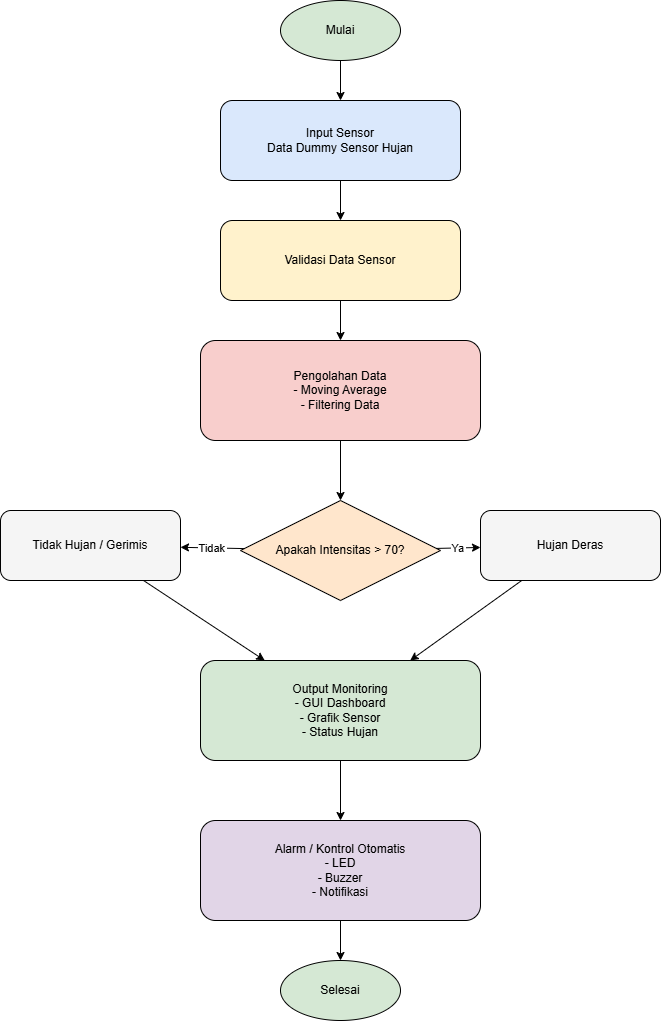
\includegraphics[width=0.9\textwidth]{flowchart.png}
    \caption{Flowchart Sistem Monitoring Hujan}
    \label{fig:flowchart}
\end{figure}

\section{Penjelasan Program Rust}

Program dibuat menggunakan:
\begin{itemize}
    \item Bahasa Rust
    \item Framework \texttt{eframe}
    \item GUI \texttt{egui}
\end{itemize}

\subsection{Struct}

\begin{lstlisting}
struct RainApp {
    rain_value: f32,
    status: String,
    history: Vec<f32>,
}
\end{lstlisting}

Struct digunakan untuk menyimpan data monitoring.

\subsection{Fungsi Validasi}

\begin{lstlisting}
fn validate_sensor(value: f32) -> f32 {
    if value < 0.0 {
        0.0
    } else if value > 100.0 {
        100.0
    } else {
        value
    }
}
\end{lstlisting}

Fungsi digunakan untuk memastikan data sensor valid.

\section{Konsep OOP}

Konsep OOP yang digunakan:

\subsection{Struct}

Rust menggunakan \texttt{struct} sebagai penyimpan data.

\subsection{Impl}

\begin{lstlisting}
impl Default for RainApp
\end{lstlisting}

Digunakan untuk mengimplementasikan fungsi pada struct.

\subsection{Method}

\begin{lstlisting}
fn update(&mut self)
\end{lstlisting}

Method digunakan untuk memperbarui GUI dan data sensor.

\section{Implementasi Komputasi Numerik}

Metode numerik yang digunakan adalah Moving Average.

\subsection{Rumus Moving Average}

\[
MA = \frac{x_1 + x_2 + x_3 + ... + x_n}{n}
\]

Keterangan:
\begin{itemize}
    \item $x$ = data sensor
    \item $n$ = jumlah data
    \item $MA$ = nilai rata-rata
\end{itemize}

\subsection{Implementasi Program}

\begin{lstlisting}
fn moving_average(data: &Vec<f32>) -> f32 {
    let mut total = 0.0;

    for value in data {
        total += value;
    }

    total / data.len() as f32
}
\end{lstlisting}

Moving Average digunakan untuk:
\begin{itemize}
    \item Mengurangi noise
    \item Menghaluskan data sensor
    \item Membuat pembacaan lebih stabil
\end{itemize}

\section{Hasil Pengujian}

Hasil pengujian dilakukan menggunakan data dummy sensor.

\begin{table}[H]
\centering
\begin{tabular}{|c|c|c|}
\hline
Data Sensor & Moving Average & Status \\ \hline
20 & 25 & Tidak Hujan \\ \hline
45 & 40 & Gerimis \\ \hline
85 & 78 & Hujan Deras \\ \hline
\end{tabular}
\caption{Hasil Pengujian Sistem}
\end{table}

GUI berhasil menampilkan:
\begin{itemize}
    \item Status hujan
    \item Grafik realtime
    \item Nilai sensor
    \item Moving Average
\end{itemize}

\section{Analisis Hasil}

Berdasarkan hasil pengujian:
\begin{itemize}
    \item Sistem mampu membaca data sensor dummy dengan baik
    \item GUI berjalan realtime
    \item Moving Average berhasil mengurangi fluktuasi data
    \item Validasi data mencegah error pembacaan
    \item Sistem alarm dapat digunakan untuk peringatan hujan deras
\end{itemize}

Kelebihan sistem:
\begin{itemize}
    \item GUI interaktif
    \item Struktur program modular
    \item Mudah dikembangkan
\end{itemize}

Kekurangan sistem:
\begin{itemize}
    \item Masih menggunakan data dummy
    \item Belum terhubung sensor asli
\end{itemize}

\section{Kesimpulan}

Berdasarkan hasil percobaan yang dilakukan dapat disimpulkan bahwa:
\begin{enumerate}
    \item Rust dapat digunakan untuk membuat GUI monitoring instrumentasi
    \item Sistem monitoring hujan berhasil dibuat menggunakan data dummy
    \item Konsep OOP pada Rust berhasil diterapkan
    \item Moving Average berhasil digunakan sebagai metode numerik
    \item Sistem dapat dikembangkan menjadi monitoring IoT realtime
\end{enumerate}

\vspace{2cm}

\begin{center}
\textbf{Terima kasih}
\end{center}

\end{document}